% !TEX root = SystemTemplate.tex

\chapter{Overview and concept of operations}

The purpose of this project is to develop a virtual reality environment that accurately represents the Ruth Brennan art exhibit at the Dahl Arts Center.  The end product will be able to be transported to and from the museum too allow students and others, who otherwise cannot visit the museum, to experience the Dahl.

The end goal for this particular project is to have the prototype gallery running through the Oculus Rift.  This is so the Dahl Arts Center can get an accurate grasp of how this sort of technology will work and will inform their decision about whether to go further with the Oculus or not.  This leads to another goal for the project team, research additional methods to utilize the virtual reality of the Oculus and give the Dahl a better understanding of what is feasible and what is fantasy.

The system that is going to be used for this project uses the Unreal Engine for the environment and the Oculus Rift for the virtual reality immersion.  In order to allow users to experience this virtual gallery, there will have to be an operator who will know how to setup the Oculus and additional software for the tour to run efficiently.  

\section{Scope}
The purpose of this document is to explain what pieces are going into this project, as well as how to install and run them.

\section{Deliverables}

\begin{enumerate}
\item Gallery room with art pieces and guided tour.  This will be the finished product that is the main purpose for this project.
\item Research into other tour methods and ideas to help the Dahl think of different ways to bring their art center out into the community.
\end{enumerate}

\section{Purpose}
The purpose of this product is to be able to take the Dahl Art Center out into the community so people who might otherwise be unable to see it, can do so.  This particular project is a proof of concept that a virtual tour is possible and will be used as a basis for future projects.


\subsection{Unreal Engine}
The Unreal Engine is the main graphics engine behind the virtual tour.  It was chosen of the Unity engine because of the level of control and detail that is necessary for rendering an art gallery. 

\subsection{Oculus Rift}
The main virtual reality product that will be used to immerse the user in the gallery.

\section{Systems Goals}
Briefly describe the overall goals this system plans to achieve.
These goals are typically provided by the stakeholders.  This is not
intended to be a detailed requirements listing.  Keep in mind that
this section is still part of the Overview.

\section{System Overview and Diagram}
Provide a more detailed description of the major system components
without getting too detailed.  This section should contain a
high-level block and/or flow diagram of the system highlighting the
major components.  See Figure~\ref{systemdiagram}.  This is a floating
figure environment.  \LaTeX\ will try to put it close to where it was
typeset but will not allow the figure to be split if moving it can not
happen.  Figures, tables, algorithms and many other floating
environments are automatically numbered and placed in the appropriate
type of table of contents.  You can move these and the numbers will
update correctly.

\begin{figure}[tbh]
\begin{center}
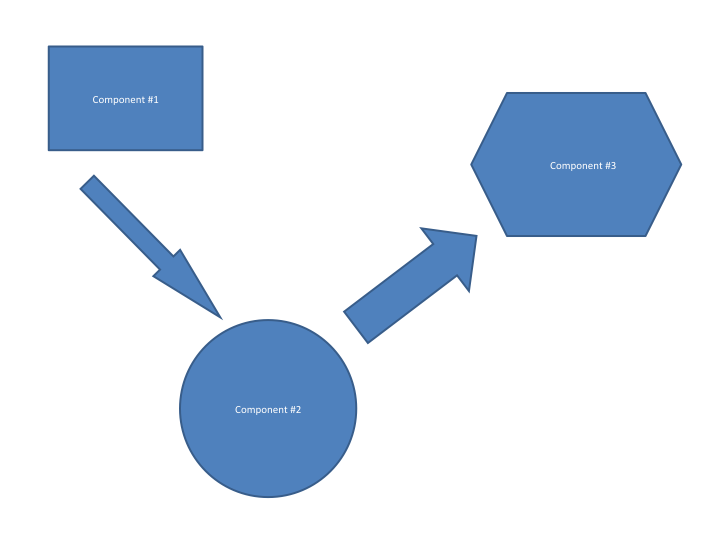
\includegraphics[width=0.75\textwidth]{./diagram}
\end{center}
\caption{A sample figure .... System Diagram \label{systemdiagram}}
\end{figure}

\section{Technologies Overview}
This section should contain a list of specific technologies used to
develop the system.  The list should contain the name of the
technology, brief description, link to reference material for further
understanding, and briefly how/where/why it was used in the system.
See Table~\ref{somenumbers}.  This is a floating table environment.
\LaTeX\ will try to put it close to where it was typeset but will not
allow the table to be split.

\begin{table}[tbh]
\caption{A sample Table ... some numbers. \label{somenumbers}}
\begin{center}
\begin{tabular}{|r|l|}
  \hline
  7C0 & hexadecimal \\
  3700 & octal \\ \cline{2-2}
  11111000000 & binary \\
  \hline \hline
  1984 & decimal \\
  \hline
\end{tabular}
\end{center}
\end{table}

